
One avenue for testing quartic gauge boson interactions is through
inclusive tri-boson production: $pp \to VV^{\prime}V^{\prime\prime}$
for $V= \gamma, W, Z$.  Using the Run 1 data sample, the triply heavy
such channels ($WWW, WWZ, WZZ, ZZZ$) are not accessible anywhere near
SM rates, due to their small 8 TeV cross sections and comparably large
multi-lepton backgrounds. The photonic channels do not suffer as much
from these problems, and sensitivity is at or near SM rates in Run 1. 

An ATLAS analysis~\cite{Aad:2015uqa} has found evidence for
$W\gamma\gamma$ production.  In this process, a $W$ is produced in the
hard quark scattering, and the two photons can originate from either
initial- or final-state radiation, or interaction with the $W$ via
triple or quartic gauge boson interactions.  Events are selected with
lepton $\pt > 20$ GeV, $\met > 25$ GeV, $m_T > 40$ GeV and two photons
with $\pt > 20$ GeV.  Minimum angular separations between the lepton
and photons are also required to reduce the contribution of
final-state radiation amplitudes, which do not probe gauge boson
interactions.  This selection results in 157 events in the 8 TeV data.
Roughly half of these events are backgrounds: $W$ or $W\gamma$ plus
jets production with jets misidentified as photons, $Z\gamma$ events
with leptons misidentified as photons, or $\gamma\gamma$ plus jets
events with jets misidentified as leptons.  The backgrounds are
estimated for electron and muon events separately via template fits to
photon isolation distributions in data ($W$ or $W\gamma$ plus jets) or
lepton isolation distributions in data ($Z\gamma$ or $\gamma\gamma$
plus jets).

The di-photon invariant mass distributions of selected events, along
with estimated backgrounds, are shown in
Fig.~\ref{fig:ss-inclboson-triboson-wgg-atlas8tev}.  A signal excess
is observed in both lepton channels, corresponding to a combined
significance larger than 3$\sigma$.  The fiducial production cross
section is estimated for both the inclusive case and an exclusive
selection with a jet veto for jets with $\pt > 30$ GeV, similar to the
ATLAS $W\gamma$ and $Z\gamma$ analysis.  The measured inclusive cross
section, $6.1^{+1.1}_{−1.0} \rm{(stat.)} \pm 1.2 \rm{(syst.)} \pm
0.2 \rm{(lumi.)}$ fb, is 1.9$\sigma$ higher than a NLO prediction from
MCFM of $2.90\pm 0.16$ fb.  The exclusive cross section,
$2.9^{+0.8}_{−0.7} \rm{(stat.)} ^{+1.0}_{−0.9} \rm{(syst.)} \pm
0.1 \rm{(lumi.)}$ fb, agrees with the MCFM prediction of $1.88\pm
0.20$ fb.  A similar phenomenon was observed in the $W\gamma/Z\gamma$
analysis, where it is believed missing higher order corrections to the
inclusive cross section are substantial.  Systematic uncertainties for
these cross sections are predominantly from the data-driven background
estimation methods.

\begin{figure}[p]
    \centering
    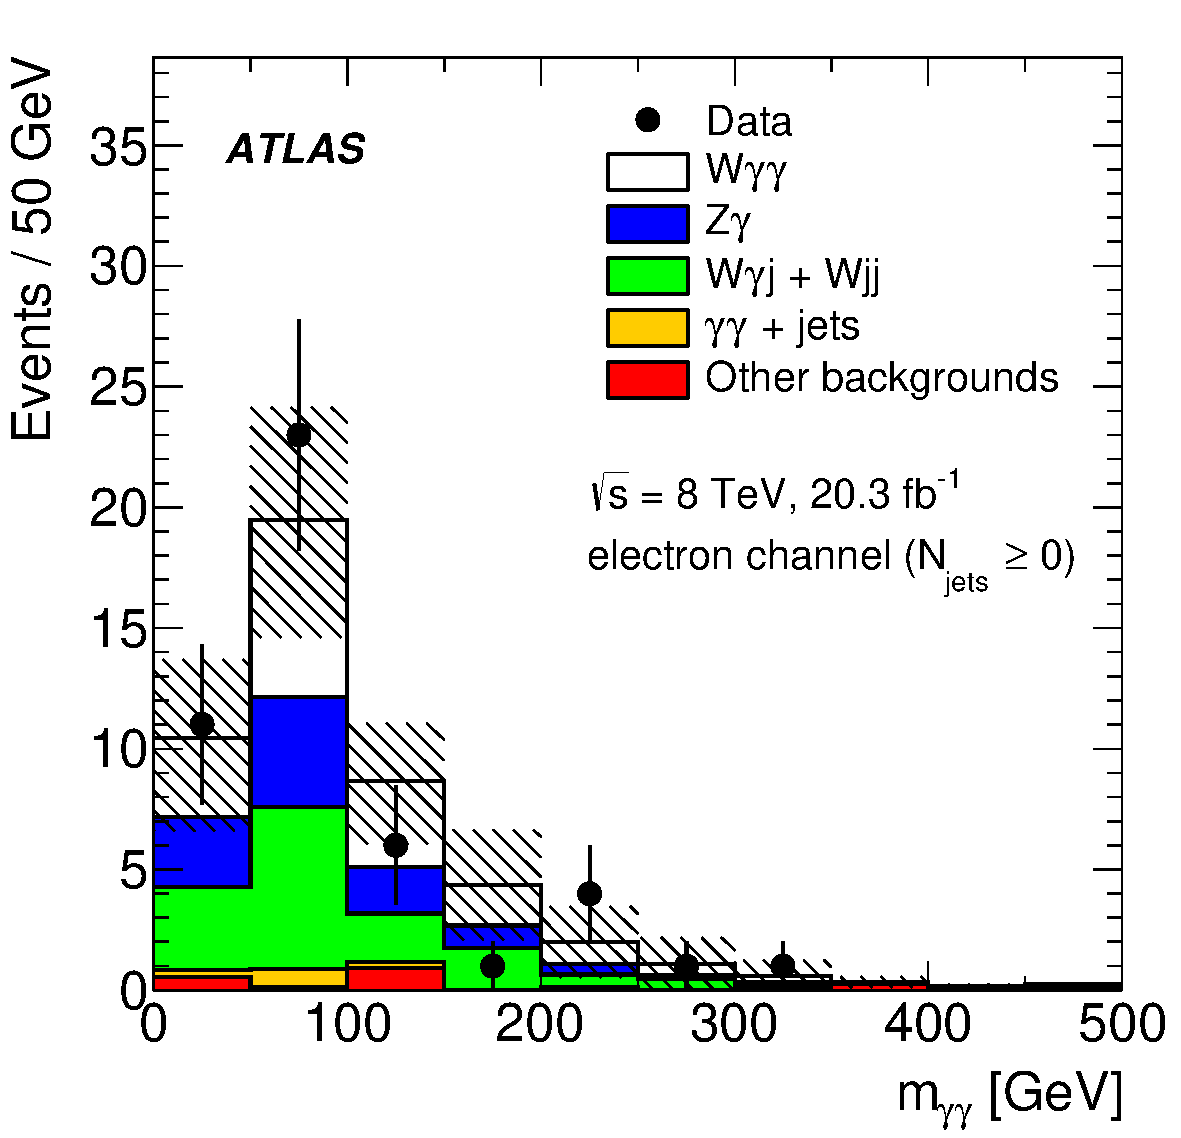
\includegraphics[width=0.45\textwidth]{figures/ss-inclboson-triboson-wgg-ele-atlas8tev.pdf}
    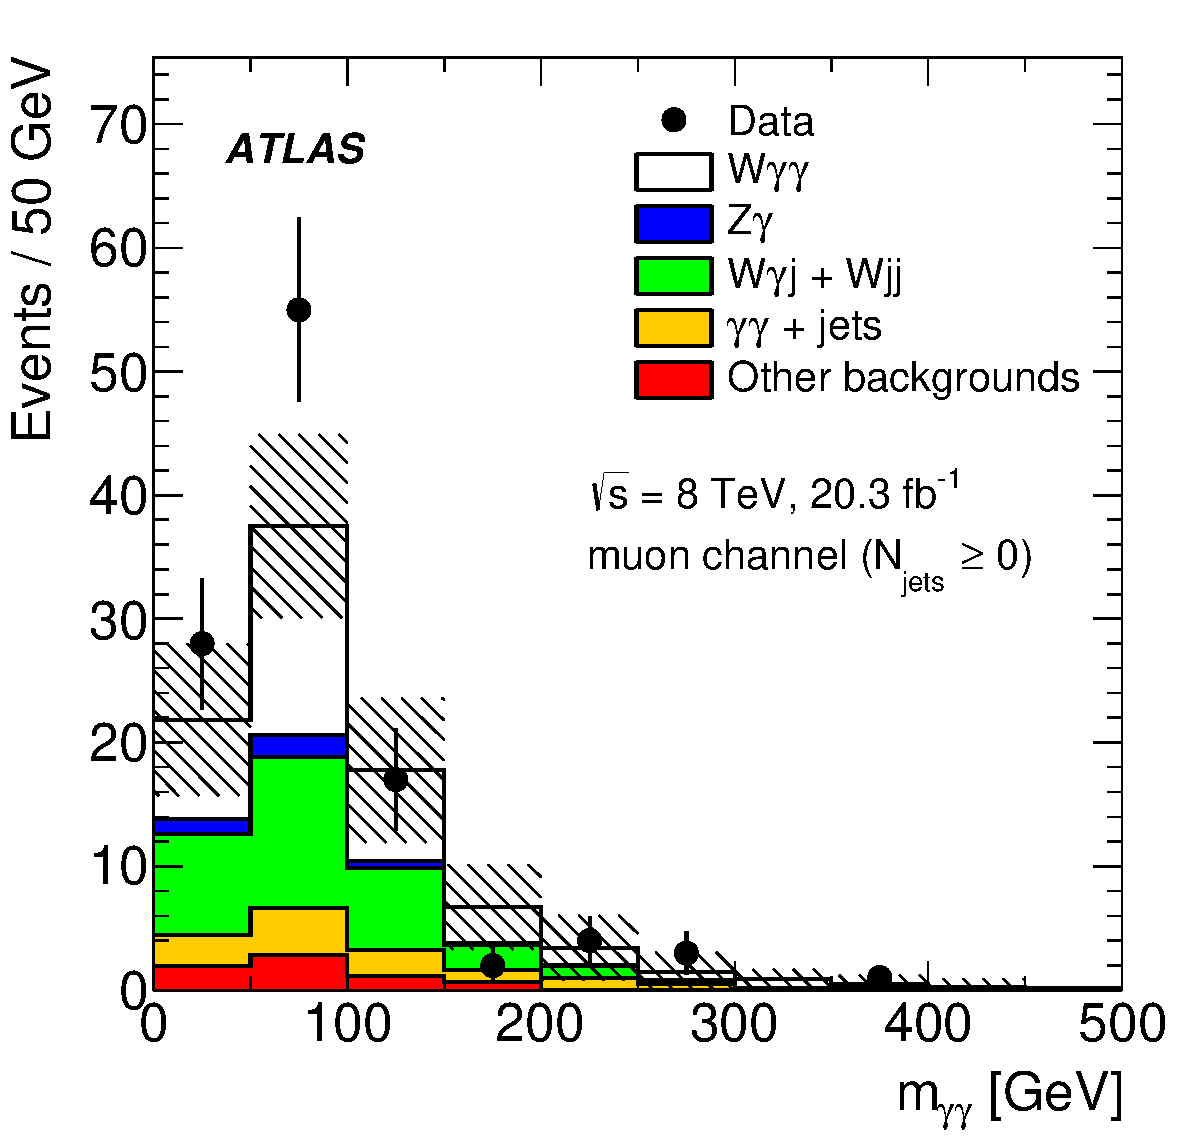
\includegraphics[width=0.45\textwidth]{figures/ss-inclboson-triboson-wgg-mu-atlas8tev.pdf}
    \caption{Di-photon invariant mass distribution of $W\gamma\gamma$ candidates selected by ATLAS~\cite{Aad:2015uqa}.  Inclusive $e\nu\gamma\gamma$ (left) and $\mu\nu\gamma\gamma$ (right) candidates are shown separately.}
    \label{fig:ss-inclboson-triboson-wgg-atlas8tev}
\end{figure}

The exclusive $W\gamma\gamma$ event yield at high di-photon mass
($m_{\gamma\gamma} > 300$ GeV) is used to obtain 95\% CL bounds on
dimension 8 EFT couplings $f_{T,0}$ and
$f_{M,(2,3)}$~\cite{Eboli:2006wa}.  For the case of no unitarizing
form factor, the observed limit on $|f_{T,0}/\Lambda^4|$ is 90
TeV$^{-4}$.  For a unitarizing form factor with a cutoff scale of 600
GeV, these limits are relaxed by up to a factor of 8.

CMS has performed a search for $WV\gamma$ production in 8 TeV
data~\cite{Chatrchyan:2014bza}, where $V$ is a hadronically decaying
$W$ or $Z$.  This process is sensitive to the $WW\gamma\gamma$ and
$WWZ\gamma$ quartic gauge boson interactions, as depicted in
Fig.~\ref{fig:ss-inclboson-triboson-wvg-diagrams}.  $W$ candidates are
selected by requiring either one muon ($\pt > 25$ GeV and
$|\eta|<2.1$) or one electron ($\pt > 30$ GeV and $|\eta| < 2.5$),
missing transverse energy in excess of 35 GeV, and vetoes on
additional leptons with $\pt > 10 (20)$ GeV for muons (electrons).
Photon candidates are required to have $\ET > 30$ GeV and $|\eta| <
1.44$; the central $\eta$ restriction selects for higher purity
photons.  The third $V$ boson is selected from jet pairs with jet $\ET
> 30$ GeV and $|\eta| < 2.4$, a veto on $b$-quark jet tags, di-jet
separation $|\Delta\eta_{jj}| < 1.4$, and di-jet mass $70 < m_{jj} <
100$ GeV.  False missing energy is reduced by requiring a minimum
azimuthal separation $|\Delta\phi| < 0.4$ between the highest $\ET$
jet and $\MET$, and false photon backgrounds from $Z$ bosons in the
electron channel are reduced by vetoing electron-photon pairs
consistent with the $Z$ mass ($|M_Z-m_{e\gamma}| < 10$ GeV).

\begin{figure}[p]
    \centering
    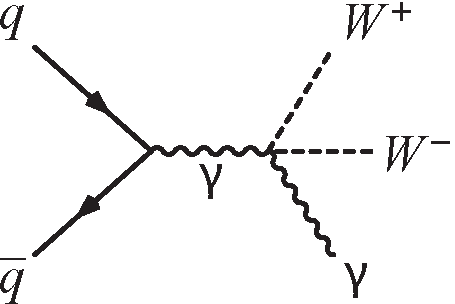
\includegraphics[width=0.3\textwidth]{figures/ss-inclboson-triboson-wvg-diagram1.pdf}
    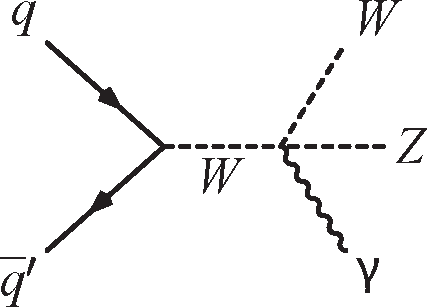
\includegraphics[width=0.3\textwidth]{figures/ss-inclboson-triboson-wvg-diagram2.pdf}
    \caption{Quartic gauge boson interaction Feynman diagrams for $WW\gamma$ and $WZ\gamma$ production~\cite{Chatrchyan:2014bza}.}
    \label{fig:ss-inclboson-triboson-wvg-diagrams}
\end{figure}


The photon $\ET$ of selected events is shown in
Fig.~\ref{fig:ss-inclboson-triboson-wvg-cms8tev}.  The leading
background is from $W\gamma$+jets production and is estimated from
extrapolation of the $m_{jj}$ sideband data into the signal region.
Multi-jet background is extrapolated from a control sample with low
$\MET$, and the other backgrounds such as top quarks are estimated
from simulation.  322 events are observed where $342\pm 16$ were
expected, of which 13 were expected to come from $WV\gamma$
production.  An upper limit at 95\% confidence level is obtained of
311 fb for the inclusive cross section, which is 3.4 times larger than
the standard model prediction of \texttt{aMC@NLO} ($91.6 \pm 21.7$ fb).

\begin{figure}[p]
    \centering
    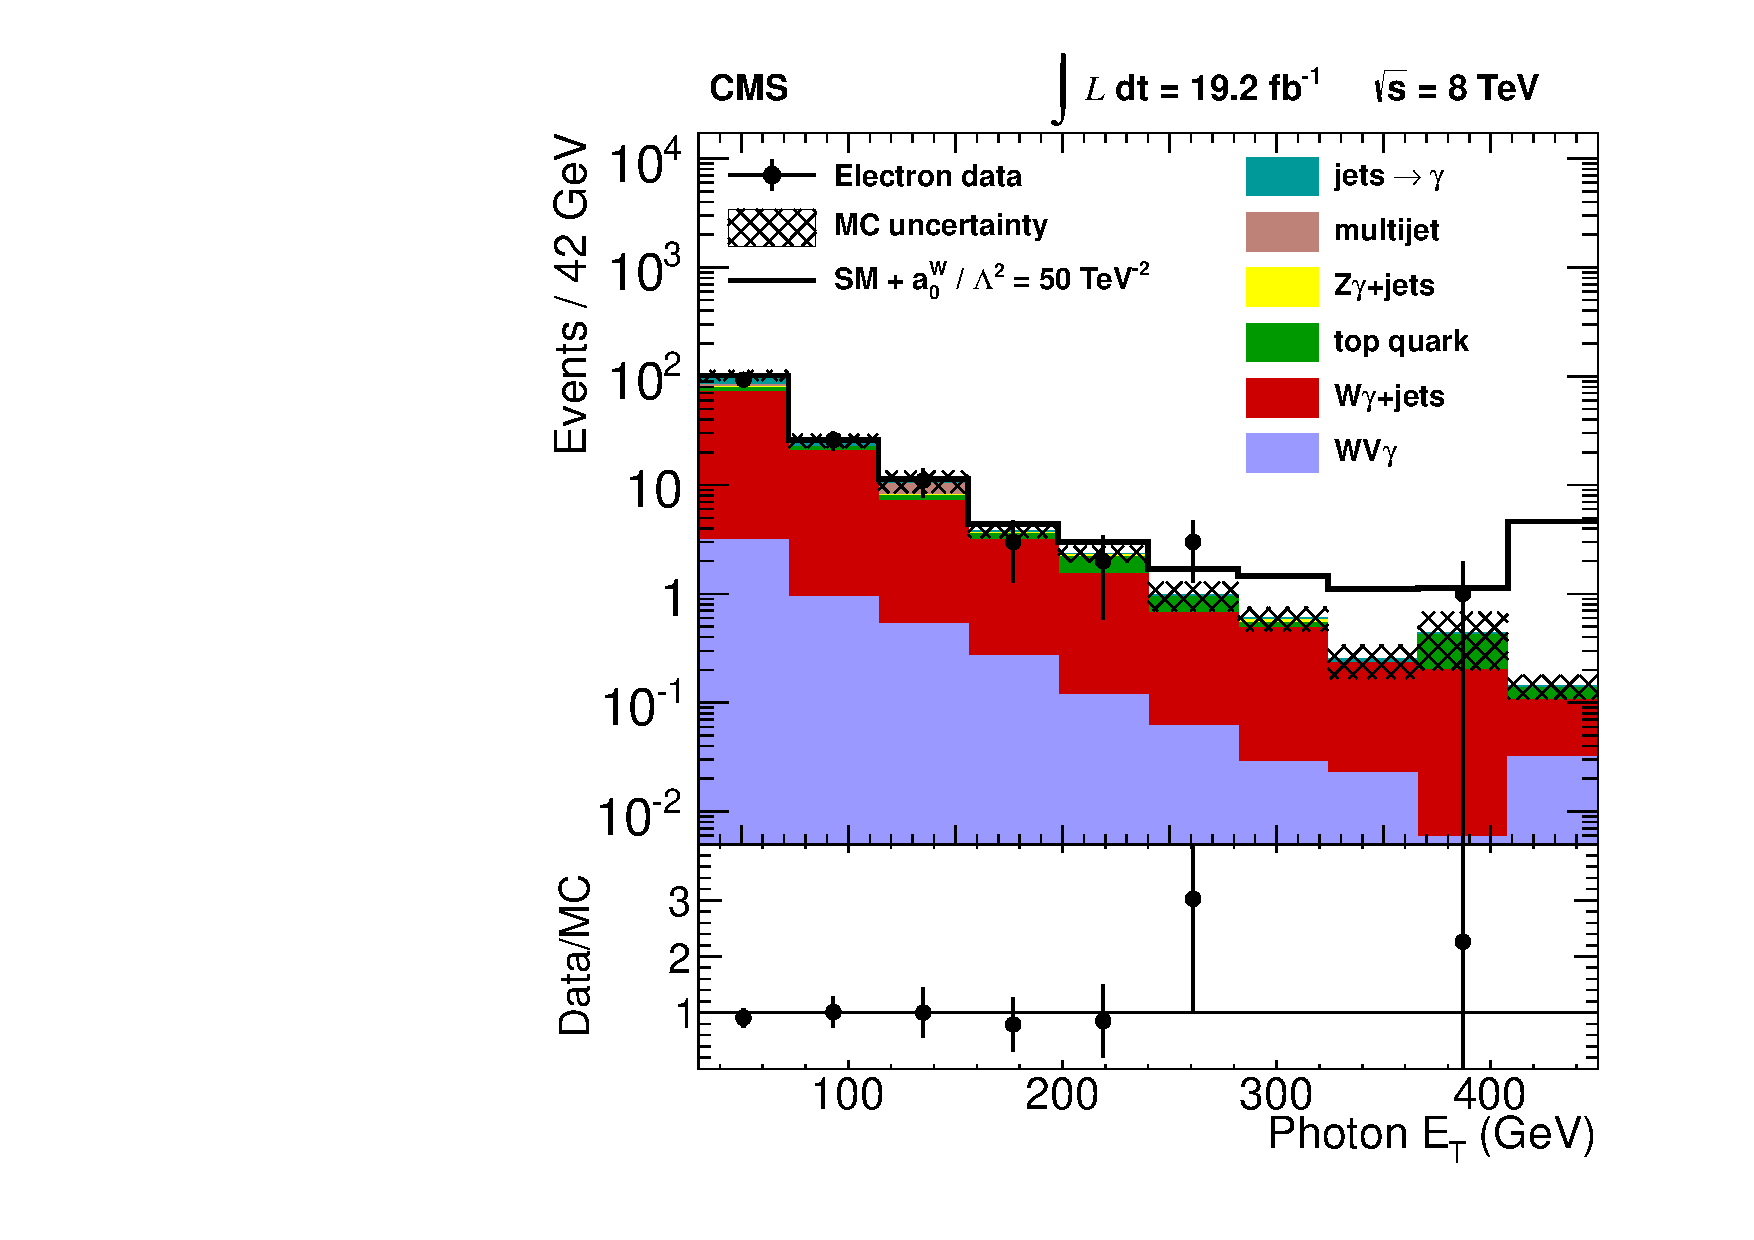
\includegraphics[width=0.45\textwidth]{figures/ss-inclboson-triboson-wvg-ele-cms8tev.pdf}
    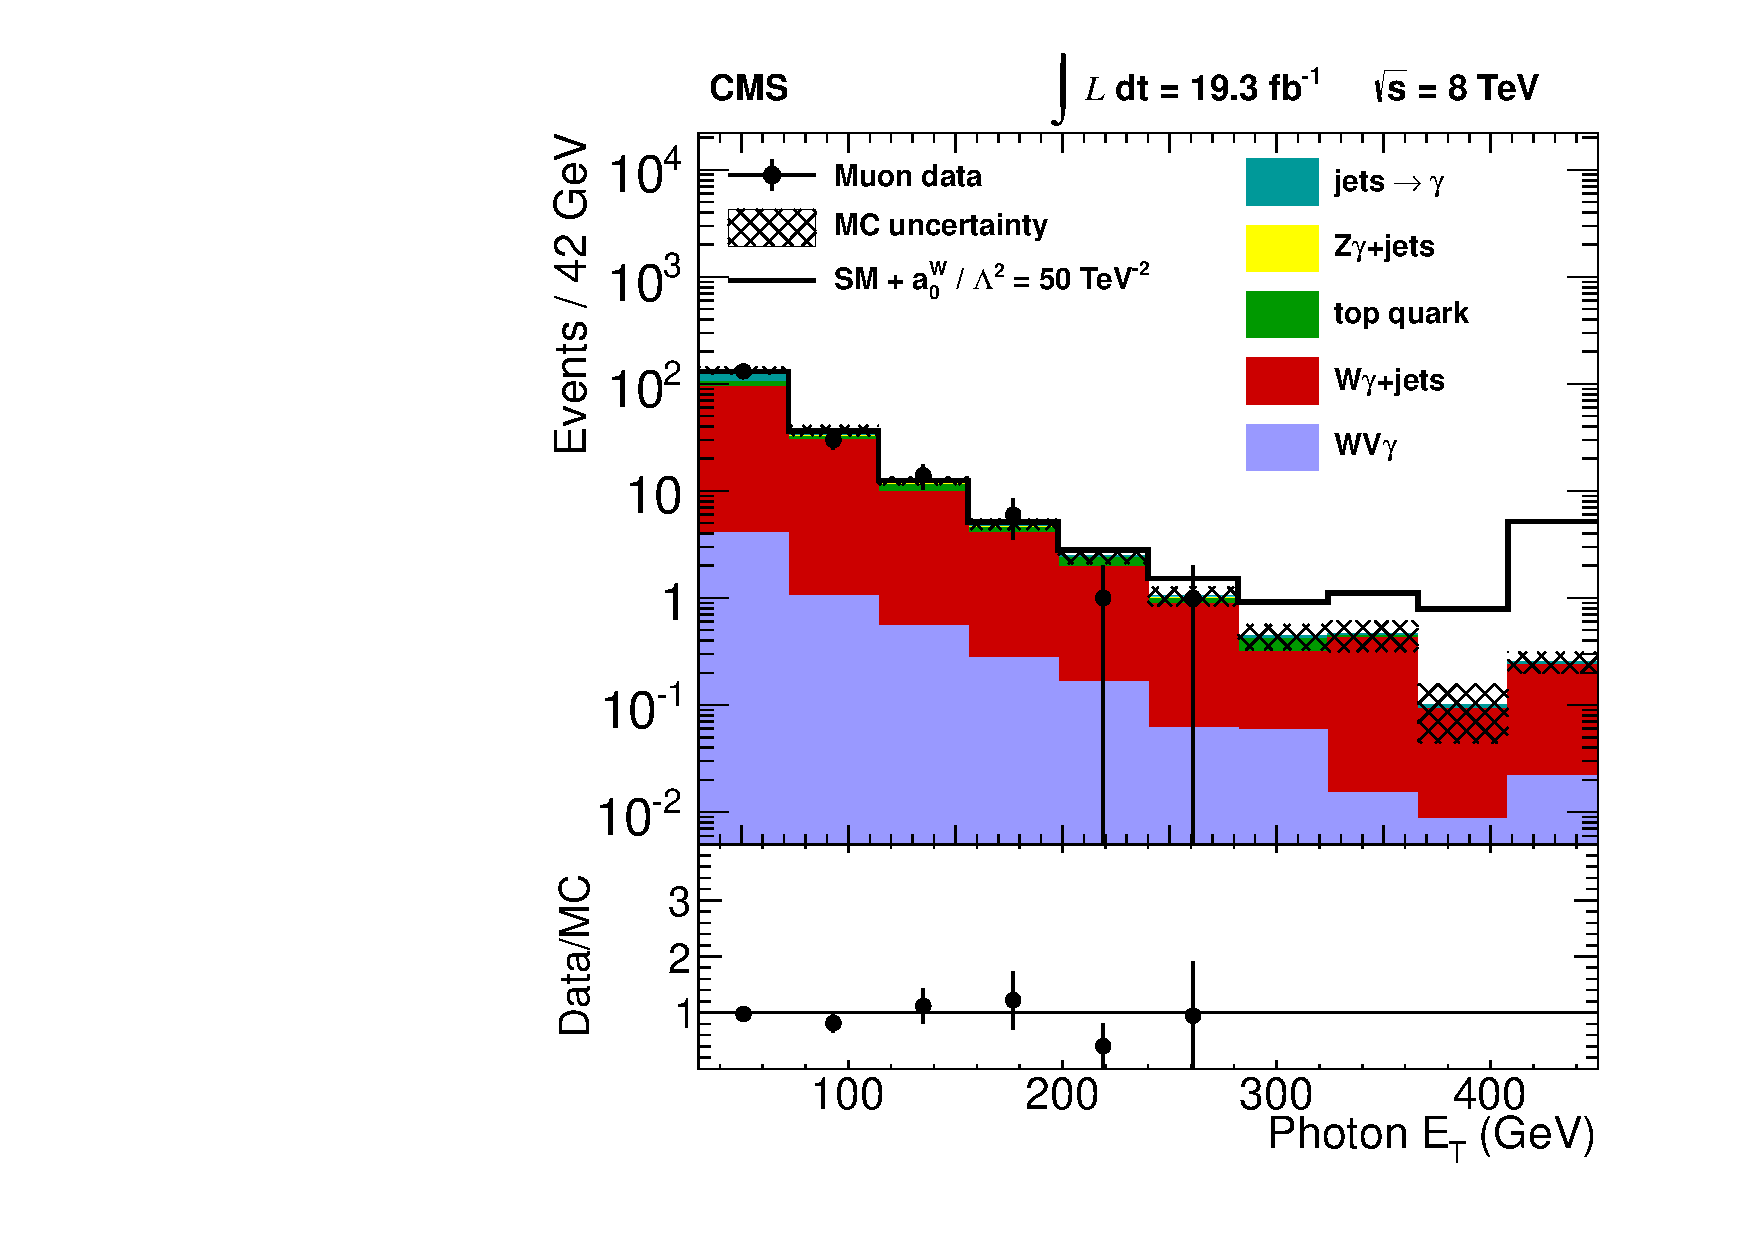
\includegraphics[width=0.45\textwidth]{figures/ss-inclboson-triboson-wvg-mu-cms8tev.pdf}
    \caption{Photon $\et$ distribution of $WV\gamma$ candidates selected by CMS~\cite{Chatrchyan:2014bza}.}
    \label{fig:ss-inclboson-triboson-wvg-cms8tev}
\end{figure}

The binned photon $\ET$ distribution in
Fig.~\ref{fig:ss-inclboson-triboson-wvg-cms8tev} is used to extract
limits on dimension 6 EFT couplings $a^W_0/\Lambda^2$ and
$a^W_C/\Lambda^2$, which affect $WW\gamma\gamma$ interactions, and
$\kappa^W_0/\Lambda^2$ and $\kappa^W_C/\Lambda^2$, which affect
$WWZ\gamma$ interactions.  The magnitude of the limits are in the
range of $12\ \textrm{TeV}^{-2}$ to $34\ \textrm{TeV}^{-2}$.  Limits
on the dimension 8 EFT couplings $f_{T,0}/\Lambda^4$,
$f_{M,0}/\Lambda^4$, $f_{M,1}/\Lambda^4$, $f_{M,2}/\Lambda^4$, and
$f_{M,3}/\Lambda^4$ are also obtained, in the range of
$25\ \textrm{TeV}^{-4}$ for $f_{T,0}/\Lambda^4$ and
$40-131\ \textrm{TeV}^{-4}$ for $f_{M,i}/\Lambda^4$.  
